% Author: Izaak Neutelings (July 2017)
% Timelines & energy scales of particle physics
% Uploaded to: https://tikz.net/timeline/
\documentclass[border=1pt,tikz]{standalone}
\usepackage{amsmath} % for \dfrac
\usepackage{tikz}
\tikzset{>=latex} % for LaTeX arrow head

% UNSLANT
% https://tex.stackexchange.com/questions/145926/upright-greek-font-fitting-to-computer-modern
% https://tex.stackexchange.com/questions/236915/adjust-custom-made-upright-greek-letters-when-used-in-subscripts
\usepackage{scalerel}
\newsavebox{\foobox}
\newcommand{\slantbox}[2][0]{\mbox{%
        \sbox{\foobox}{#2}%
        \hskip\wd\foobox
        \pdfsave
        \pdfsetmatrix{1 0 #1 1}%
        \llap{\usebox{\foobox}}%
        \pdfrestore
}}
\newcommand\unslant[2][-.25]{%
  \mkern1.2mu%
  \ThisStyle{\slantbox[#1]{$\SavedStyle#2$}}%
  \mkern-1.2mu%
}
\newcommand\unslantlong[2][-.25]{% % for long letter like mus
  \mkern-0.2mu%
  \ThisStyle{\slantbox[#1]{$\SavedStyle#2$}}%
  \mkern-0.8mu%
}
\newcommand{\upalpha}{\unslant\alpha}
\newcommand{\upgamma}{\unslant\gamma}
\newcommand{\upeta}{\unslant\eta}
\newcommand{\upmu}{\unslantlong\mu}
\newcommand{\upnu}{\unslant\nu}
\newcommand{\uppi}{\unslant\pi}
\newcommand{\uprho}{\unslant\rho}
\newcommand{\uptau}{\unslant\tau}
\newcommand{\upphi}{\unslantlong\phi}
\newcommand{\upchi}{\unslantlong\chi}
\newcommand{\uppsi}{\unslant\psi}
\newcommand{\upomega}{\unslant\omega}
\newcommand{\Jpsi}{\ensuremath{\mathrm{J}\mspace{-2mu}/\mspace{-2mu}\uppsi}} % J/psi meson

\begin{document}



%% TIMELINE - simple test
%\begin{tikzpicture}[]
%  
%  % USER SETTINGS
%  \newcount\yearOne; \yearOne=1900
%  \def\w{15}    % width of axes
%  \def\n{4}     % number of decades
%  \def\lt{0.33} %  ten tick length
%  \def\lf{0.28} % five tick length
%  \def\lo{0.24} %  one tick length
%  
%  % HELP FUNCTION
%  \def\yearLabel(#1,#2){\node[above] at ({(#1-\yearOne)*\w/\n/10},\lt) {#2};}
%  \def\yearArrowLabel(#1,#2,#3,#4){ % year, yoffset, ylength, label
%    \pgfmathsetmacro\xy{(#1-\yearOne)*\w/\n/10}
%    \pgfmathsetmacro\drawbelow{#2<0}
%    \ifnum \drawbelow=1 % draw below timeline
%      \pgfmathsetmacro\yyp{\lt*(0.90+#2)}
%      \pgfmathsetmacro\yyw{\yyp-\lt*#3}
%      \draw[<-,thick,black,align=center] (\xy,\yyp) -- (\xy,\yyw) node[below,black] at (\xy,\yyw) {#4};
%    \else % draw above timeline
%      \pgfmathsetmacro\yyp{\lt*(0.10+#2)}
%      \pgfmathsetmacro\yyw{\yyp+\lt*#3}
%      \draw[<-,thick,black,align=center] (\xy,\yyp) -- (\xy,\yyw) node[above,black] at (\xy,\yyw) {#4};
%    \fi}
%  
%  % AXIS
%  %\draw[thick] (0,0) -- (\w,0);
%  \draw[->,thick] (-\w*0.03,0) -- (\w*1.03,0);
%  
%  % TICKS
%  \foreach \tick in {0,1,...,\n}{
%    \def\x{{\tick*\w/\n}}
%    \def\year{\the\numexpr \yearOne+\tick*10 \relax}
%  	\draw[thick] (\x,\lt) -- (\x,-\lt) % ten tick
%	             node[below] {\year};
%	
%	\ifnum \tick<\n
%	  \draw[thick] ({(\x+\w/\n/2)},0) -- ({(\x+\w/\n/2)},\lf); % five tick
%      \foreach \ticko in {1,2,3,4,6,7,8,9}{
%        \def\xo{{(\x+\ticko*\w/\n/10)}}
%  	    \draw[thick] (\xo,0) -- (\xo,\lo);  % one tick
%	}\fi
%  }
%  
%  % label
%  \yearLabel(1923,lol)
%  \yearArrowLabel(1932.2, 1.0,1.0,foo)
%  \yearArrowLabel(1937.2, 1.0,1.5,foo bar)
%  \yearArrowLabel(1907.5, 0.0,1.5,small)
%  \yearArrowLabel(1915.6,-1.0,2.0,\small this is small a sentence)
%  \yearArrowLabel(1924.2,-1.2,1.2,$p\lambda=h$)
%  
%\end{tikzpicture}



% LOGARITHMIC ENERGY SCALE
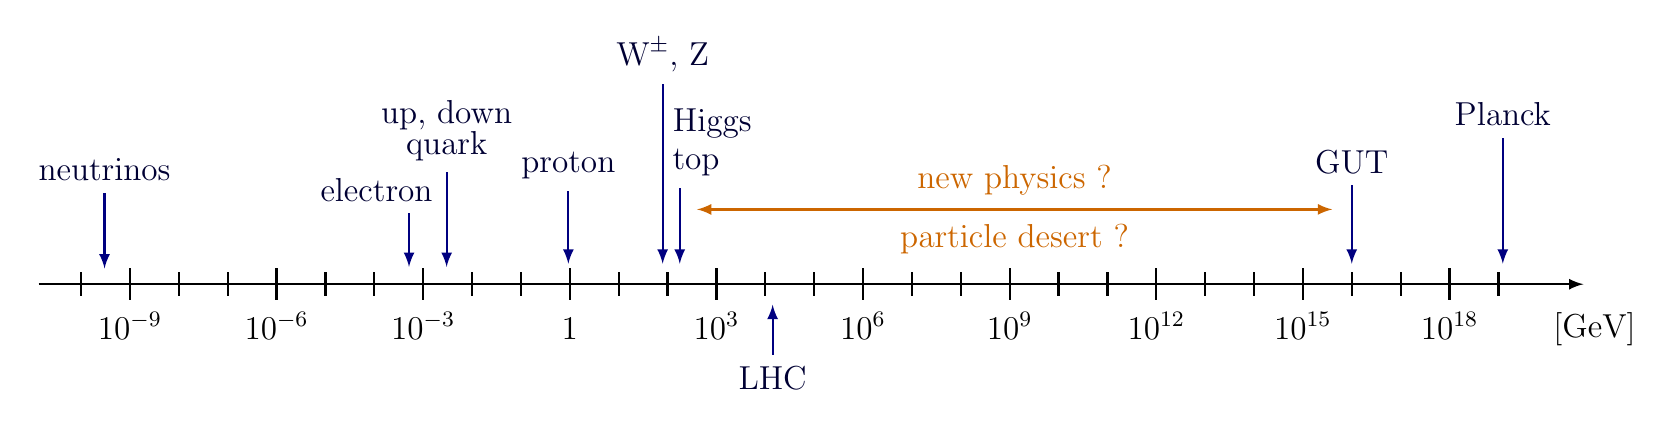
\begin{tikzpicture}
  \large
  
  % USER SETTINGS
  \newcount\nOne; \nOne=-10
  \def\w{18}      % width of axes
  \def\n{29}      % number of decades
  \def\noffset{1} % offset labels
  \def\nskip{3}   % skip number
  \def\la{2.00}   % arrow length
  \def\lt{0.20}   % tick length
  \def\ls{0.15}   % tick length (skipped)
  
  % HELP FUNCTION
  \def\myx(#1){{(#1-\nOne)*\w/\n}}
  \def\arrowLabel(#1,#2,#3,#4){ % log10(xpos), yoffset, ylength, label
    \pgfmathsetmacro\drawbelow{#2<0}
    \ifnum \drawbelow=1 % draw below line
      \pgfmathsetmacro\yyp{(\lt*(-0.10+#2))}
      \pgfmathsetmacro\yyw{(\yyp-\la*\lt*#3)}
      \draw[<-,thick,black!50!blue,align=center]
        (\myx(#1),\yyp) -- (\myx(#1),\yyw)
        node[below,black!80!blue] {#4}; %,fill=white
    \else % draw above line
      \pgfmathsetmacro\yyp{(\lt*(0.10+#2)}
      \pgfmathsetmacro\yyw{(\yyp+\la*\lt*#3)}
      \draw[<-,thick,black!50!blue,align=center]
        (\myx(#1),\yyp) -- (\myx(#1),\yyw)
        node[above,black!80!blue] {#4};
    \fi
  }
  %\def\arrowLabelRed(#1,#2,#3,#4){
  %  \def\yyp{{(\lt*(-0.10+#2))}}; \def\yyw{{(\yyp-\la*\lt*#3)}}
  %  \fill[red,radius=2pt] (\myx(#1),0) circle;
  %  \draw[<-,thick,black!25!red,align=center]
  %    (\myx(#1),\yyp) -- (\myx(#1),\yyw)
  %    node[below,black!40!red] {\strut#4}; %,fill=white
  %}
  
  % AXIS
  \draw[->,thick] (-\w*0.03,0) -- (\w*1.06,0)
                  node[right=4pt,below=6pt] {[GeV]};
  
  % TICKS
  \foreach \tick in {0,1,...,\n}{
    \def\x{{\tick*\w/\n}}
    \def\dec{\the\numexpr \nOne+\tick \relax}
	\pgfmathsetmacro\tentick{Mod(\tick-\noffset,\nskip)==0}
	\ifnum\tentick=1
	  \draw[thick] (\x,\lt) -- (\x,-\lt) node[below] { % ten tick
	                 \ifnum\dec=0 \strut$1$
	                 \else \strut$10^{\dec}$ \fi
	               }; % label
	\else
      \draw[thick] (\x,\ls) -- (\x,-\ls); % ten tick
	\fi
  }
  
  % LABELS
  \arrowLabel(-9.52,0.9,2.4,neutrinos)      % log(0.0000000003)=-9.523 (0.3 eV)
  \arrowLabel(-2.52,1.0,3.0,up, down\\[-3pt]quark) % log(0.003)=-2.523 (~3 MeV)
  \arrowLabel(-3.29,1.0,1.7,electron\qquad) % log(0.000510)=-3.292 (0.510 MeV)
  %\arrowLabel(-0.98,1.2,1.5,muon\;\;)       % log(0.1057)=-0.976 (105.7 MeV)
  \arrowLabel(-0.03,1.2,2.3,proton)         % log(0.938)=-0.03
  \arrowLabel( 1.90,1.2,5.7,$\text{W}^\pm$, $\text{Z}$) % log(80)=1.90, log(90)=1.95
  \arrowLabel( 2.25,1.2,2.4,\qquad Higgs\\\quad top)    % log(125)=2.10, log(175)=2.24
  \arrowLabel( 4.15,-1.2,1.6,LHC)           % log(1400)=4.146 (14 TeV)
  \arrowLabel(16.00,1.2,2.5,GUT)            % 10^25 eV = 10^16 GeV
  \arrowLabel(19.09,1.2,4.0,Planck)         % Planck (quantum gravity) 1.9561e9*6.2415e9 GeV = 1.22e19 GeV
  
  % low mass boson & vector-like bottom quark
  %\arrowLabelRed(1.477,-1.2,3.0,X)    % ln(30) = 1.477
  %\arrowLabelRed(2.230,-1.2,3.0,$\text{B}'$) % ln(170) = 2.230
  
  % STRETCH
  \draw[<->,thick,black!20!orange]
    ({(2.6-\nOne)*\w/\n},0.95) -- ({(15.6-\nOne)*\w/\n},0.95)
    node[midway,below=1pt] {particle desert ?}
    node[midway,above=1pt] {new physics ?};
  
\end{tikzpicture}



%% LOGARITHMIC ENERGY & LENGTH SCALE
%\begin{tikzpicture}
%  \large
%  
%  % USER SETTINGS
%  \newcount\nOne; \nOne=-10
%  \def\w{18}      % width of axes
%  \def\n{29}      % number of decades
%  \def\noffset{1} % offset labels
%  \def\nskip{3}   % skip number
%  \def\la{2.00}   % arrow length
%  \def\lt{0.20}   % tick length with label
%  \def\ls{0.14}   % tick length without label
%  
%  % HELP FUNCTION
%  \def\myx(#1){{(#1-\nOne)*\w/\n}}
%  \def\arrowLabel(#1,#2,#3,#4){ % log10(xpos), yoffset, ylength, label
%    \pgfmathsetmacro\drawbelow{#2<0}
%    \ifnum \drawbelow=1 % draw below line
%      \pgfmathsetmacro\yyp{(\lt*(-0.10+#2))}
%      \pgfmathsetmacro\yyw{(\yyp-\la*\lt*#3)}
%      \draw[<-,thick,black!50!blue,align=center]
%        (\myx(#1),\yyp) -- (\myx(#1),\yyw)
%        node[below,black!80!blue] {#4}; %,fill=white
%    \else % draw above line
%      \pgfmathsetmacro\yyp{(\lt*(0.10+#2)}
%      \pgfmathsetmacro\yyw{(\yyp+\la*\lt*#3)}
%      \draw[<-,thick,black!50!blue,align=center]
%        (\myx(#1),\yyp) -- (\myx(#1),\yyw)
%        node[above,black!80!blue] {#4};
%    \fi
%  }
%  
%  % AXES
%  \draw[->,thick] (-\w*0.03,0) -- (\w*1.06,0)
%                  node[right=4pt,above=6pt] {[GeV]};
%  % AXES
%  \draw[->,thick] (\w*1.06,-4*\lt) -- (-\w*0.03,-4*\lt)
%                  node[right=4pt,below=6pt] {[cm]};
%  
%  % TICKS
%  \foreach \tick in {0,1,...,\n}{
%    \def\x{{\tick*\w/\n}}
%    \def\dec{\the\numexpr \nOne+\tick \relax}
%	\pgfmathsetmacro\tentick{Mod(\tick-\noffset,\nskip)==0}
%	\ifnum\tentick=1
%	  \draw[thick] (\x,\lt) -- (\x,-\lt) node[below] { % ten tick
%	                 \ifnum\dec=0 \strut$1$
%	                 \else \strut$10^{\dec}$ \fi
%	               }; % label
%	\else
%      \draw[thick] (\x,\ls) -- (\x,-\ls); % ten tick
%	\fi
%  }
%  
%  % LABELS
%  \arrowLabel(-9.52,0.9,2.4,neutrinos)      % log(0.0000000003)=-9.523 (0.3 eV)
%  \arrowLabel(-2.52,1.0,3.0,up, down\\[-3pt]quark) % log(0.003)=-2.523 (~3 MeV)
%  \arrowLabel(-3.29,1.0,1.7,electron\qquad) % log(0.000510)=-3.292 (0.510 MeV)
%  %\arrowLabel(-0.98,1.2,1.5,muon\;\;)       % log(0.1057)=-0.976 (105.7 MeV)
%  \arrowLabel(-0.03,1.2,2.3,proton)         % log(0.938)=-0.03
%  \arrowLabel( 1.90,1.2,5.7,$\text{W}^\pm$, $\text{Z}$) % log(80)=1.90, log(90)=1.95
%  \arrowLabel( 2.25,1.2,2.4,\qquad Higgs\\\quad top)    % log(125)=2.10, log(175)=2.24
%  \arrowLabel( 4.15,-1.2,1.6,LHC)           % log(1400)=4.146 (14 TeV)
%  \arrowLabel(16.00,1.2,2.5,GUT)            % 10^25 eV = 10^16 GeV
%  \arrowLabel(19.09,1.2,4.0,Planck)         % Planck % quantum gravity % 1.22x10^19 . GeV
%  
%  % STRETCH
%  \draw[<->,thick,black!20!orange]
%    ({(2.6-\nOne)*\w/\n},0.95) -- ({(15.6-\nOne)*\w/\n},0.95)
%    node[midway,below=1pt] {particle desert ?}
%    node[midway,above=1pt] {new physics ?};
%  
%\end{tikzpicture}



% TIMELINE - particle physics
% sources: http://web.ihep.su/dbserv/compas/src/
%          http://www.particleadventure.org/other/history/
%          https://en.wikipedia.org/wiki/Timeline_of_particle_discoveries
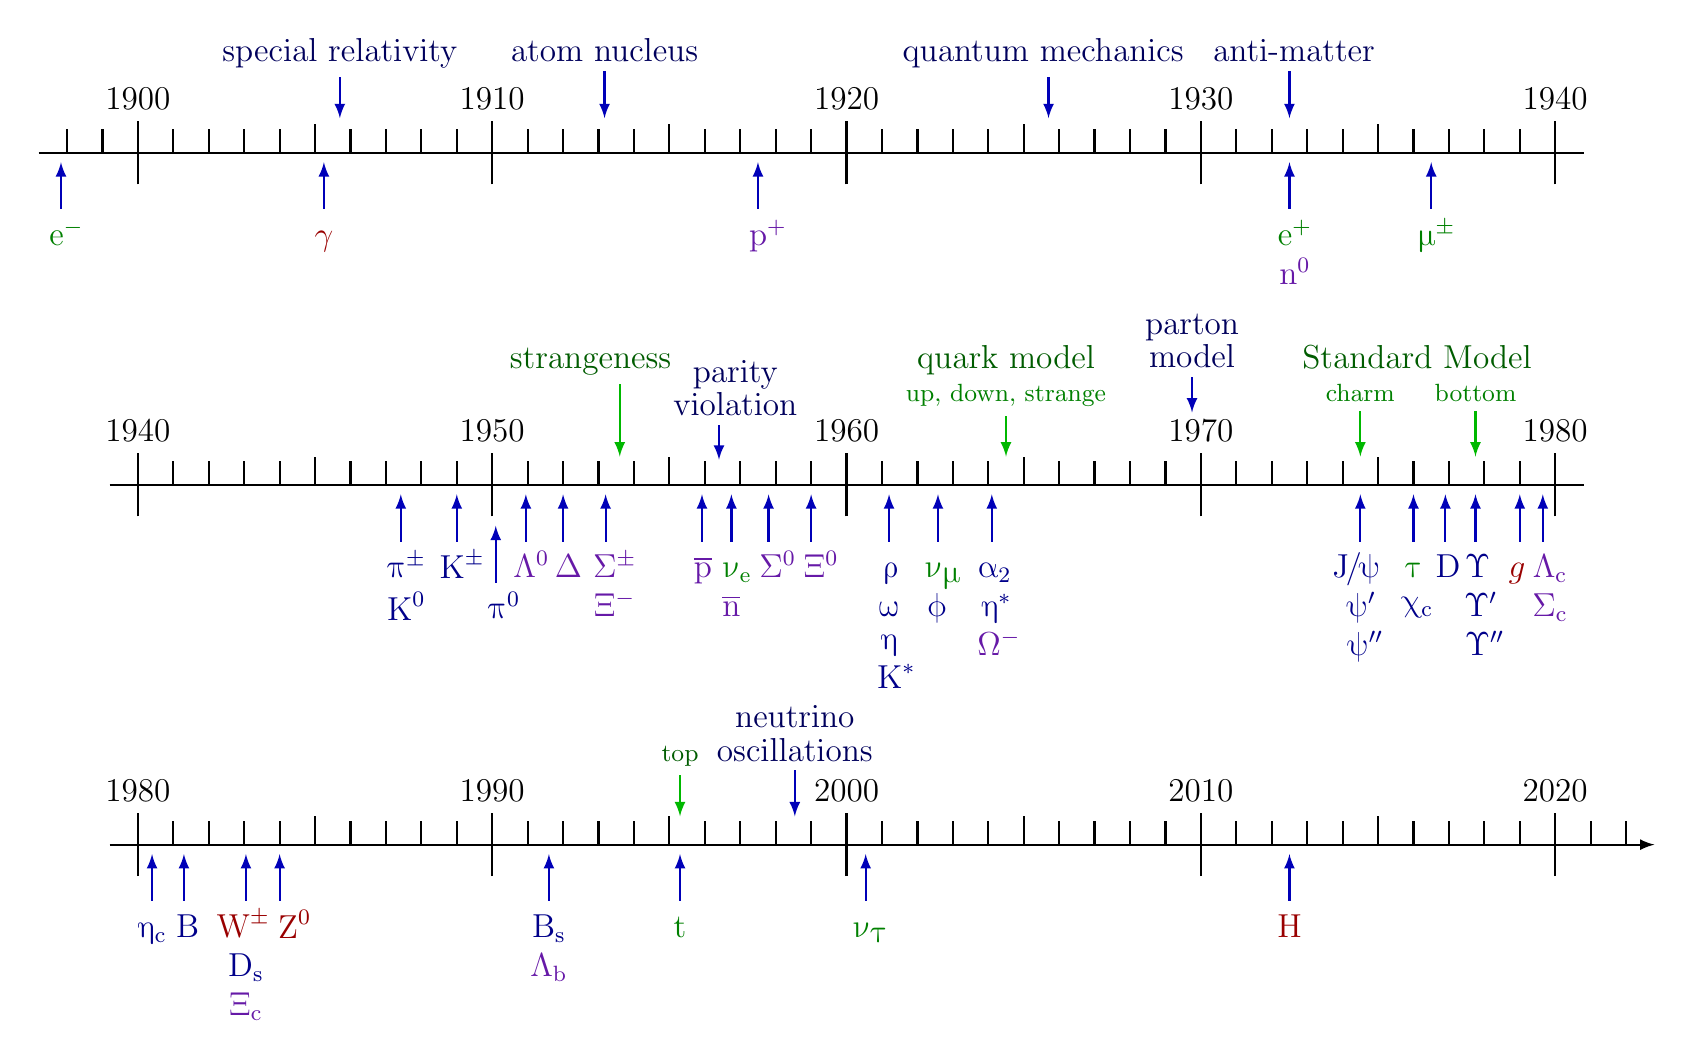
\begin{tikzpicture}%[minimum height=10pt, text height=10pt,text depth=10pt,
  \large
  
  % USER SETTINGS
  \newcount\yearOne; \yearOne=1900
  \newcount\yoffset;
  \def\w{18}       % width of axes
  \def\n{4}        % number of decades per row
  \def\lt{0.40}    %  ten tick length
  \def\lf{0.36}    % five tick length
  \def\lo{0.30}    %  one tick length
  \def\lext{0.07}  % left extension of axes
  \def\rext{1.02}  % right extension of axes
  \colorlet{myblue}{blue!90!black}
  \colorlet{mygreen}{green!90!black}
  \def\fermtxt#1{\color{green!50!black}#1} % fermion (green)
  \def\ferm#1{$\fermtxt{#1}$} % fermion (green)
  \def\boson#1{$\color{red!60!black}#1$} % boson (red)
  \def\baryon#1{$\color{blue!65!red!95!black!90}#1$} % baryon (purple)
  
  % HELP FUNCTION
  \def\axis[#1]{
  
    % AXIS
    \def\rextlocal{#1} % local right extension of axes
    \pgfmathsetmacro\drawarrow{\rextlocal>1.045}
    \ifnum \drawarrow=1 % draw below timeline
      \draw[->,thick] (-\w*\lext,0) -- (\w*\rextlocal,0);
    \else
      \draw[thick] (-\w*\lext,0) -- (\w*\rextlocal,0);
    \fi
    
    % TICKS
    \pgfmathsetmacro\ydensity{(10*\n)/\w} % number of years / length
    \pgfmathsetmacro\ymin{int(ceil(\yearOne-\w*\lext*\ydensity))}
    \pgfmathsetmacro\ymax{int(floor(\yearOne+\w*(\rextlocal-0.003)*\ydensity))}
    \foreach \year [evaluate={%
      \x=(\year-\yearOne)/\ydensity; % x position
      \m=( mod(\year,10)==0 ? 10 : (mod(\year,5)==0 ? 5 : 1) ); % 10, 5, or 1 tick
    }] in {\ymin,...,\ymax}{
      \ifnum \m=10 % ten tick
        \draw[thick] (\x,-\lt) -- (\x,\lt) node[above] {\year};
      \fi
      \ifnum \m=5 % five tick
        \draw[thick] (\x,0) -- (\x,\lf);
      \else % one tick
        \draw[thick] (\x,0) -- (\x,\lo);
      \fi
    }
    
  }
  \def\yearArrowLabelCol[#1](#2,#3,#4,#5){
    \def\xy{{(#2-\yearOne)*\w/\n/10}}
    \pgfmathsetmacro\drawbelow{#3<0}
    \ifnum \drawbelow=1 % draw below timeline
      \pgfmathsetmacro\yyp{\lt*(0.90+#3)}
      \pgfmathsetmacro\yyw{\yyp-\lt*#4}
      \draw[<-,thick,black!20!#1,align=center]
        (\xy,\yyp) -- (\xy,\yyw)
        node[below=-1pt,black!40!#1] at (\xy,\yyw) {\strut #5};
    \else % draw below timeline
      \pgfmathsetmacro\yyp{\lt*(0.10+#3)}
      \pgfmathsetmacro\yyw{\yyp+\lt*#4}
      \draw[<-,thick,black!20!#1,align=center]
        (\xy,\yyp) -- (\xy,\yyw)
        node[above=-1pt,black!60!#1] at (\xy,\yyw) {#5};
    \fi
  }
  \def\yearArrowLabel(#1,#2,#3,#4){\yearArrowLabelCol[myblue](#1,#2,#3,#4)}
  \def\yearArrowLabelGreen(#1,#2,#3,#4){\yearArrowLabelCol[mygreen](#1,#2,#3,#4)}
  \def\yearArrowLabelRed(#1,#2,#3,#4){
    \yearArrowLabelCol[red](#1,#2,#3,#4)
    \fill[red,radius=2pt] (\xy,0) circle;
  }
  \def\yearLabel(#1,#2,#3){
    \node[above,below,black!60!mygreen] at ({(#1-\yearOne)*\w/\n/10},{\lt*#2}) {#3};
  }
  
  
  %---------------%
  %  1900 - 1940  %
  %---------------%
  
  % AXIS
  \axis[\rext]
  
  % LABELS
  \yearArrowLabel(1897.83,-1.2,1.5,
    \ferm{\text{e}^-})     % 10/1897 Thomson (electron)
  \yearArrowLabel(1905.25,-1.2,1.5,%
    \boson{\gamma})        % 03/1905 Einstein (photon)
  \yearArrowLabel(1905.70,1.0,1.3,%
    special relativity)    % 09/1905 Einstein
  \yearArrowLabel(1913.17,1.0,1.5,
    atom nucleus)          % 02/1913 Rutherford (nucleus)
  \yearArrowLabel(1917.50,-1.2,1.5,
    \;\baryon{\text{p}^+}) % 1917 Rutherford, Philos. Mag., Ser. 6, Vol. 37, 581 (1919) (proton)
  \yearArrowLabel(1925.70,1.0,1.3,%
    \!\!quantum mechanics) % 09/1925 Schrodinger equation
  \yearArrowLabel(1932.50,-1.2,1.5,%
    \ \ferm{\text{e}^+}\\  % 1932 Anderson (positron)
    \ \baryon{\text{n}^0}) % 1932 Chadwick (neutron)
  \yearArrowLabel(1932.50,1.0,1.5,
    \;anti-matter)         % 1932 anti-matter (previously predicted by Dirac)
  \yearArrowLabel(1936.50,-1.2,1.5,
    \ferm{\upmu^\pm})      % 1936 (muon)
  
  
  %---------------%
  %  1940 - 1980  %
  %---------------%
  
  \yearOne=1940; \advance\yoffset by 120
  \def\lext{0.02} % reset left extension of axes
  \begin{scope}[yshift=-\yoffset]
    
    % AXIS
    \axis[\rext]
    
    % LABELS
    \yearArrowLabel(1947.42,-1.2,1.5,
      $\uppi^\pm$\\              % pions    05/1947 Lattes, Muirhead, Occhialini, Powell
    \ $\text{K}^0$)              % neutral kaons 12/1947 Rochester & Butler, Nature, 160, 855
    \yearArrowLabel(1949.00,-1.2,1.5,
      $\text{K}^\pm$)            % kaons    12/1949 Powell, Fowler, Perkins, Nature, 163, 82
    \yearArrowLabel(1950.10,-2.2,1.8,
    \,$\uppi^0$)                 % pi0      01/1950 Caltech
    \yearArrowLabel(1950.95,-1.2,1.5,
      \baryon{\Lambda^0})        % Lambda0  12/1950 Hopper, Biswas, Phys. Rev. 80, 1099
    \yearArrowLabel(1952.00,-1.2,1.5,
      \baryon{\Delta})           % 1952 Anderson, Fermi, (Chicago Cyclotron), Phys. Rev., 85, 936
                                 % 1956 Ashkin (Rochester cyclotron), Phys. Rev., 101, 1149
    \yearArrowLabel(1953.20,-1.2,1.5,%
      \;\;\baryon{\Sigma^\pm}\\  % Sigma+ 1953 Bonetti, Nuovo Cimento, 10, 1; Danysz, Pniewski, Phil. Mag., 44, 348; Cosmotron Brookhaven, Phys. Rev., 93, 109
      \;\;\baryon{\Xi^-})        % Xi- "negative hyperon" 1954 Cowan (Caltech), Phys. Rev., 94, 161
    \yearArrowLabelGreen(1953.6,0.8,2.3,%
      strangeness\hspace{1.8em}) % 08/1953 Gell-Man, Phys. Rev. 92, 833, 1953
    \yearArrowLabel(1956.4,0.7,1.1,% 0.8,1.46
      \quad parity\\[-2pt]       % 01/1956 Wu experiment parity violation in Co
      \quad violation)           %         Physical Review. 105 (4) (1956): 1413
    \yearArrowLabel(1955.92,-1.2,1.5,
      \baryon{\overline{\text{p}}}\;) % 11/1955 Chamberlain, Segrè (Bevatron) Phys. Rev. 100, 947
    \yearArrowLabel(1956.75,-1.2,1.5,
      \ferm{\upnu_\text{e}}\\    %
      \baryon{\overline{\text{n}}}) % 09/1956 Reines, Cowan, Nature, 178, 446
    \yearArrowLabel(1957.80,-1.2,1.5,
      \:\baryon{\Sigma^0})       % 
    \yearArrowLabel(1959.00,-1.2,1.5,
      \;\baryon{\Xi^0})          % Xi 1959 (1964 Brookhaven)
    % 1960  Sigma*(1385) Phys. Rev. Lett., 5, 520
    \yearArrowLabel(1961.20,-1.2,1.5,%
      $\uprho$\\                 % 1961 Erwin (Cosmotron) Phys. Rev. Lett., 6, 628
      $\upomega$\\[-2pt]         % 1961 Maglic, Alvarez, Phys. Rev. Lett., 7, 178
      $\upeta$\\                 % 1961 Pevsner, Phys. Rev. Lett., 7, 421
      \,\;$\text{K}^*$)          % 1961 Alston, Phys. Rev. Lett., 6, 300, 1962 Phys. Rev. Lett., 9, 330
    % 19.. strangeness "associated-production", Pais
    % 1962 Eightfold Way, Gell-Man
    \yearArrowLabel(1962.58,-1.2,1.5,\vspace{2pt}
      \ferm{\upnu_{\upmu}}\\     % 07/1962, Ledderman, Danby, Phys. Rev. Lett. 9, 36
      $\upphi$)                  % 1962, Pjerrou Phys. Rev. Lett., 9, 114, Bertanza, Phys. Rev. Lett., 9, 180
    % 1962 f particle?
    \yearArrowLabel(1964.10,-1.2,1.5,%
      \,$\upalpha_2$\\           %
      \;$\upeta^*$\\             %
      \;\,\baryon{\Omega^-})     % 02/1964, Barnes, Brookhaven, Phys. Rev. Lett. 12, 204
    \yearArrowLabelGreen(1964.5,0.8,1.3,
      \small \fermtxt{up}, \fermtxt{down}, \fermtxt{strange})
    \yearLabel(1964.5,4.8,%
      quark model)               % 1964 Gell-Mann & Zweig
    \yearArrowLabel(1969.75,2.2,1.12,
      parton\\[-2pt]             % 09/1969 Feynman, Conf. Proc. C 690905 (1969), 237
      model)
    \yearArrowLabelGreen(1974.50,0.8,1.45,%
      \small\fermtxt{charm})     % charm quark
    \yearLabel(1976.1,4.8,%
      Standard Model)            % 1967 Steven Weinberg, Abdus Salam: electroweak unification
    % 1974 November Revolution
    \yearArrowLabel(1974.50,-1.2,1.5,%
      $\Jpsi\phantom{'}$\\
      \;$\uppsi'\phantom{'}$\\   % 
      \;$\uppsi''$)              % 
    \yearArrowLabel(1976.00,-1.2,1.5,%
      \ferm{\uptau}\\[-2pt]      % tau 1975 Perl, Abrams, Phys. Rev. Lett. 35, 1489
      \;$\upchi_\text{c}$)       % 
    \yearArrowLabel(1976.90,-1.2,1.5,
      $\text{D}$\,)              % 1976 SLAC
    \yearArrowLabelGreen(1977.75,0.8,1.45,
      \small\fermtxt{bottom})    % bottom quark
    \yearArrowLabel(1977.75,-1.2,1.5,%
       \;\;$\Upsilon\phantom{''}$\\ % Fermilab
       \;\;$\Upsilon'\phantom{'}$\\
       \;\;$\Upsilon''$)
       %\;\small\ldots)           % Fermilab
    \yearArrowLabel(1979.0,-1.2,1.5,%
      \boson{g}\,)                % gluon (DESY)
    \yearArrowLabel(1979.65,-1.2,1.5,%
      \;\,\baryon{\Lambda_\text{c}}\\
      \;\,\baryon{\Sigma_\text{c}}) % 
    
  \end{scope}
  
  
  %---------------%
  %  1980 - 2020  %
  %---------------%
  
  \yearOne=1980; \advance\yoffset by 130
  \begin{scope}[yshift=-\yoffset]
    
    % AXIS
    \axis[1.07]
    
    % LABELS
    \yearArrowLabel(1980.40,-1.2,1.5,%
      $\upeta_\text{c}$)       % eta
    \yearArrowLabel(1981.30,-1.2,1.5,%
      \:B)                     % B hadron
    \yearArrowLabel(1983.05,-1.2,1.5,%
      \!\boson{\text{W}^\pm}\\ % W boson
      $\text{D}_\text{s}$\\
      \baryon{\Xi_\text{c}})
    \yearArrowLabel(1984.00,-1.2,1.5,
      \hspace{7pt}\boson{\text{Z}^0}) % Z boson
    \yearArrowLabel(1991.60,-1.2,1.5,%
      $\text{B}_\text{s}$\\    % Bs Fermilab
      \baryon{\Lambda_\text{b}})
    \yearArrowLabel(1995.30,-1.2,1.5,%
      \fermtxt{\text{t}})      % top
    \yearArrowLabelGreen(1995.30,0.8,1.3,%
      \small{top})             % top
    \yearArrowLabel(1998.54,0.8,1.46,%
      neutrino\\[-2pt]         % 07/1998 Super-Kamiokande
      oscillations)            %         Phys. Rev. Lett. 81, 1562
    \yearArrowLabel(2000.54,-1.2,1.5,
      \ferm{\upnu_{\uptau}})   % tau neutrino (announced in 2000)
    \yearArrowLabel(2012.50,-1.2,1.5,%
      \boson{\text{H}})        % Higgs
    
    %% NEW PARTICLES ?
    %%\yearArrowLabelRed(2017.7,-1.2,1.5,X\\\,$\text{B}'$) % low mass
    %\yearArrowLabelRed(2023.2,-1.2,1.5,
    %  LQ ?) % leptoquark (hypothetical)
    
  \end{scope}
  
  
\end{tikzpicture}



\end{document}
